\chapter{Evaluation}
\label{chapt:evaluation}
This Chapter describes the evaluation of the scalability of the system architecture, the evaluation of the topic classification mechanism and the collaboration and contribution to user interface evaluation.  

\section{Scalability}
\label{sec:eval_scalability}
This Section describes the evaluation of the two different implementations of the system architecture. In the first architecture, more than one memcached instances at layer 2 were introduced, as figure~\ref{fig:system_architecture} shows. In the second, more than one Social Network engines were introduced at layer 1.

In order to measure the response time (RT) the Apache JMeter application~\cite{jmeter_url} is used. The Apache JMeter is an open source benchmark designed to test functional behaviour and  measure performance, targeting web applications. Notably, the RT measured by JMeter may not be the real one, because the JMeter measures the elapsed time from just before sending the request to just after the last response from the server has been received. As a result, the time to render the web page to the client web browser and the execution time of JavaScript code is not measured. Because those two time intervals are client limited and depend on client performance and on which web browser is used, they are excluded from the following performance test benches. For the next experiments, a specific web page will be used. This page does not use any AJAX call, in order to not misguide the results. Therefore, the RT measures the time from just before JMeter sends the request to just after the last response is received. During this measured time interval, the Social Network engine performs the following actions:
\begin{enumerate}[I]
\item The Social Network engine sends a request to CDO Client for the application execution model.
\item The CDO Client forwards this request to CDO Server.
\item Afterwards CDO Server queries the mysql repository of application models and executions, and finally gets the executions results.
\item CDO Server forwards the results through the CDO Client to the Social Network Engine.
\item Finally, the Social Network engine sends queries to the Social Network DB in order to get all the necessary Social features for this application page
\end{enumerate}

The presented system architecture was deployed on Amazon EC2~\cite{amazon_url} and the system CPU Utilization and the response time of SNP is measured.

\subsection{Focusing on memcached}
\label{sec:eval_memcache}
By adding a Memcached node at the system architecture, the Social Network Engine first asks the Memcached node if it has the tuples that the SN Engine needs. So the steps(\emph{I} to \emph{V}), mentioned previously, are not necessary if the Memcached node has cached the values that the Social Network Engine needs. The loop through CDO CIient - CDO Server and the repositories is bypassed. 

\begin{table}[]
\centering
\caption{Number of Queries from Social Network and CDO server repository.}
\label{tab:num_of_queries}
\begin{tabular}{ll}
State        & \# of Queries \\
Fresh start  & 1938          \\
Fresh Query  & 15182         \\
Cached Query from CDO & 251           \\
Cached Query from Memcached & 147  
\end{tabular}
\end{table} 

For the following experiments all the Memcached nodes are warmed up and have already cached all the needed CDO and Social entities information. Furthermore the CDO server has been warmed up after a fresh restart. As the table~\ref{tab:num_of_queries} shows,
the starting process of the CDO server produces 1938 queries to MySQL database. The \emph{fresh query} for an application model (both social information and executions) produces 15182 queries to MySQL database. The CDO server caches the results, so a second query for this application model produces 251 queries, most of which are the queries for the social information of the application. Introducing Memcached, if the request for the application model is cached, the queries to database are lowering to 147.  

\begin{figure}[h]
	\caption{The average response time for all configurations.}
	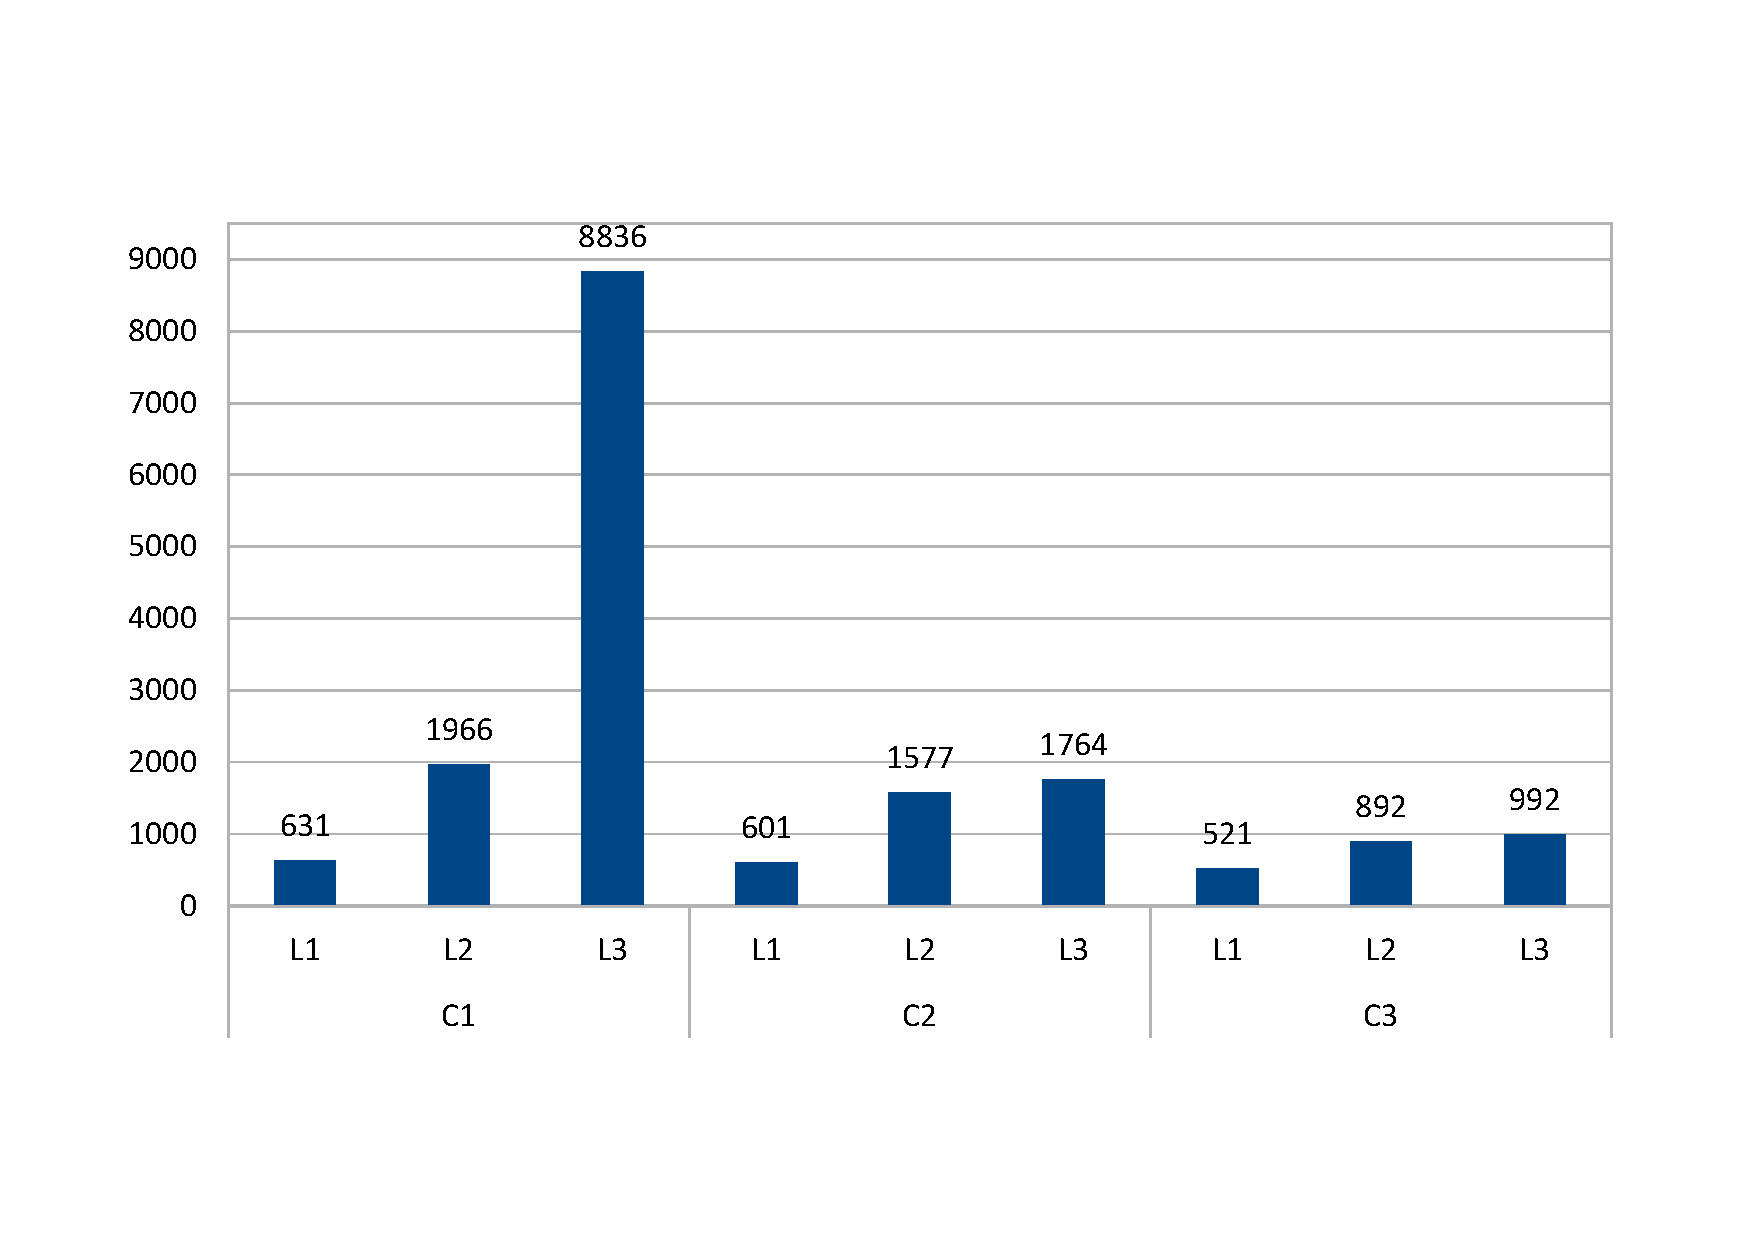
\includegraphics[width=0.9\textwidth,natwidth=200,natheight=150]{./fig/RTavg.pdf}
	\centering
	\label{fig:rtavg}
\end{figure}

The test performed with the following loads: (L1) ten users request \emph{two} applications, (L2) ten users request \emph{four} applications and (L3) ten users request \emph{eight} applications. All three Loads run consecutively one hundred times each. Those Loads request applications, which have ten execution rows pulled from the repository of applications models and executions, and about one hundred queries to the Social Network DB. In this experiment we kept the following components of the system constant: the Elgg front-end Apache2 server, the Social Network Database, and the CDO server - client communication but we increased the number of Memcached nodes.
The figure~\ref{fig:rtavg} shows the  average response time (RT) in milliseconds with the following system configuration(C): (C1) no Memcached node , (C2) one Memcached node and (C3) two Memcached nodes have added to the system architecture.

As we going from C1 to C3 and specifically for L3, the RT is reduced by 80,4\% at C2 and by 88,78\% at C3. As the figure~\ref{fig:rtavg} shows, at the first configuration C1, the L3 takes 8836 ms, an RT which is definitely prohibitive for web applications. Introducing more Memcached nodes at C2 and C3 the RT is decreased dramatically at 1764 ms at L2 and at 992 ms at L3. Going from C1 to C2, the 80,4\% reduction of RT is due to the introduction of Memcached node and bypassed the steps I - V. Going from C2 to C3, the 43,77\% reduction of RT. The reduction of RT is achieved by adding more Memcached nodes, which results to more CPU cores introduced to the architecture as described below.

\begin{figure}[h]
	\caption{The average CPU utilization for all components.}
	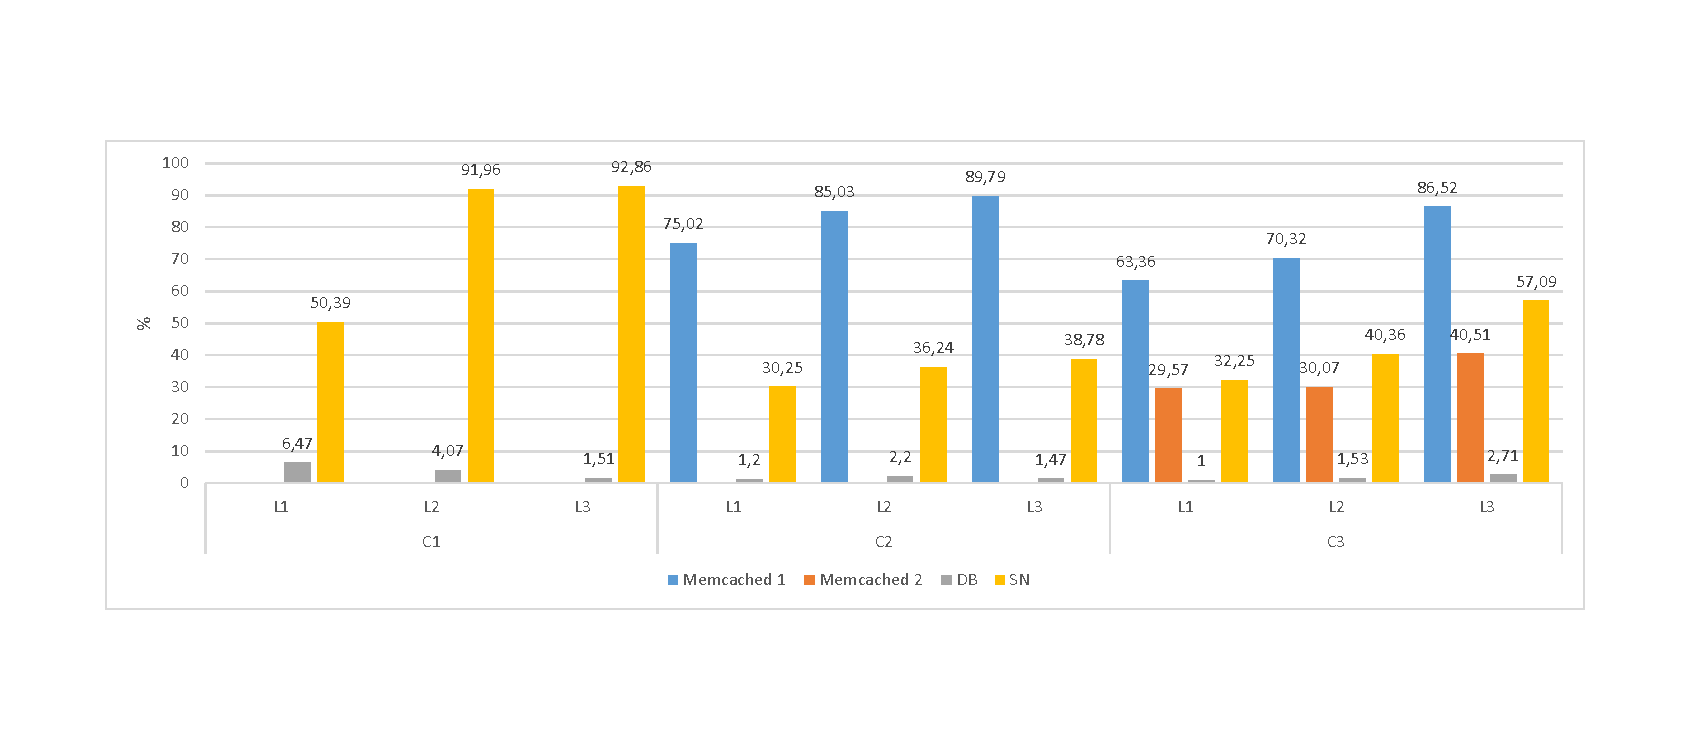
\includegraphics[width=1.1\textwidth,natwidth=200,natheight=250]{./fig/UsageAVG.pdf} 
	\centering
	\label{fig:cpuavg}
\end{figure}

The CPU utilization is measured using the sysstat tool~\cite{sysstat_url}. We measured the CPU utilization for all the VMs running the experiment. The information about the VM resources is listed in the table~\ref{vms_resources}. The Social Network Engine and the CDO Client were running at t1.micro instance. The mysql (repositories) and the CDO Server were running at m1.xlarge. The average CPU utilization is shown in the figure~\ref{fig:cpuavg}. At the simple configuration C1, even in small loads such as L1, the SN Engine reached 50,39\% CPU utilization. In the medium load L2 and big load L3 the SN Engine is kneeled down to 91,96\% and 92,86\%. This big consumption of CPU was due to all the initialization that Elgg Social Network Engine has to do for each request and due to CDO Server queries.

Moving from configuration C1 to C2, the CPU consumption went to Memcached node. Thus, the Social Network engine was de-congested and the RT improved. However, for the big load L3 the Memcached node reached 89,79\%. To solve Memcached CPU overhead, one more Memcached node was added at configuration C3. This second Memcached node shared the CPU overhead with the first Memcached node and the RT improved furthermore. 

For all three loads at C3, the first Memcached node had more CPU utilization from the second by an approximately factor of 2,2. This difference between the two Memcached nodes appeared due to the first node storing more popular key-value pairs than the other.

\begin{table}[]
\centering
\caption{VM resources. }
\label{vms_resources}
\begin{tabular}{|l|l|}
\hline
 Component &  VM type \\ \hline
 SN engine, CDO client &  t1.micro \\ \hline
 memcached &  t1.micro \\ \hline
 repositories, CDO Server &  m1.xlarge \\ \hline
 jmeter &  m1.large \\ \hline
\end{tabular}
\end{table}

\subsection{Focusing on the Elgg engine}

\begin{figure}[h]
	\caption{The Response time for two Social Network Engines.}
	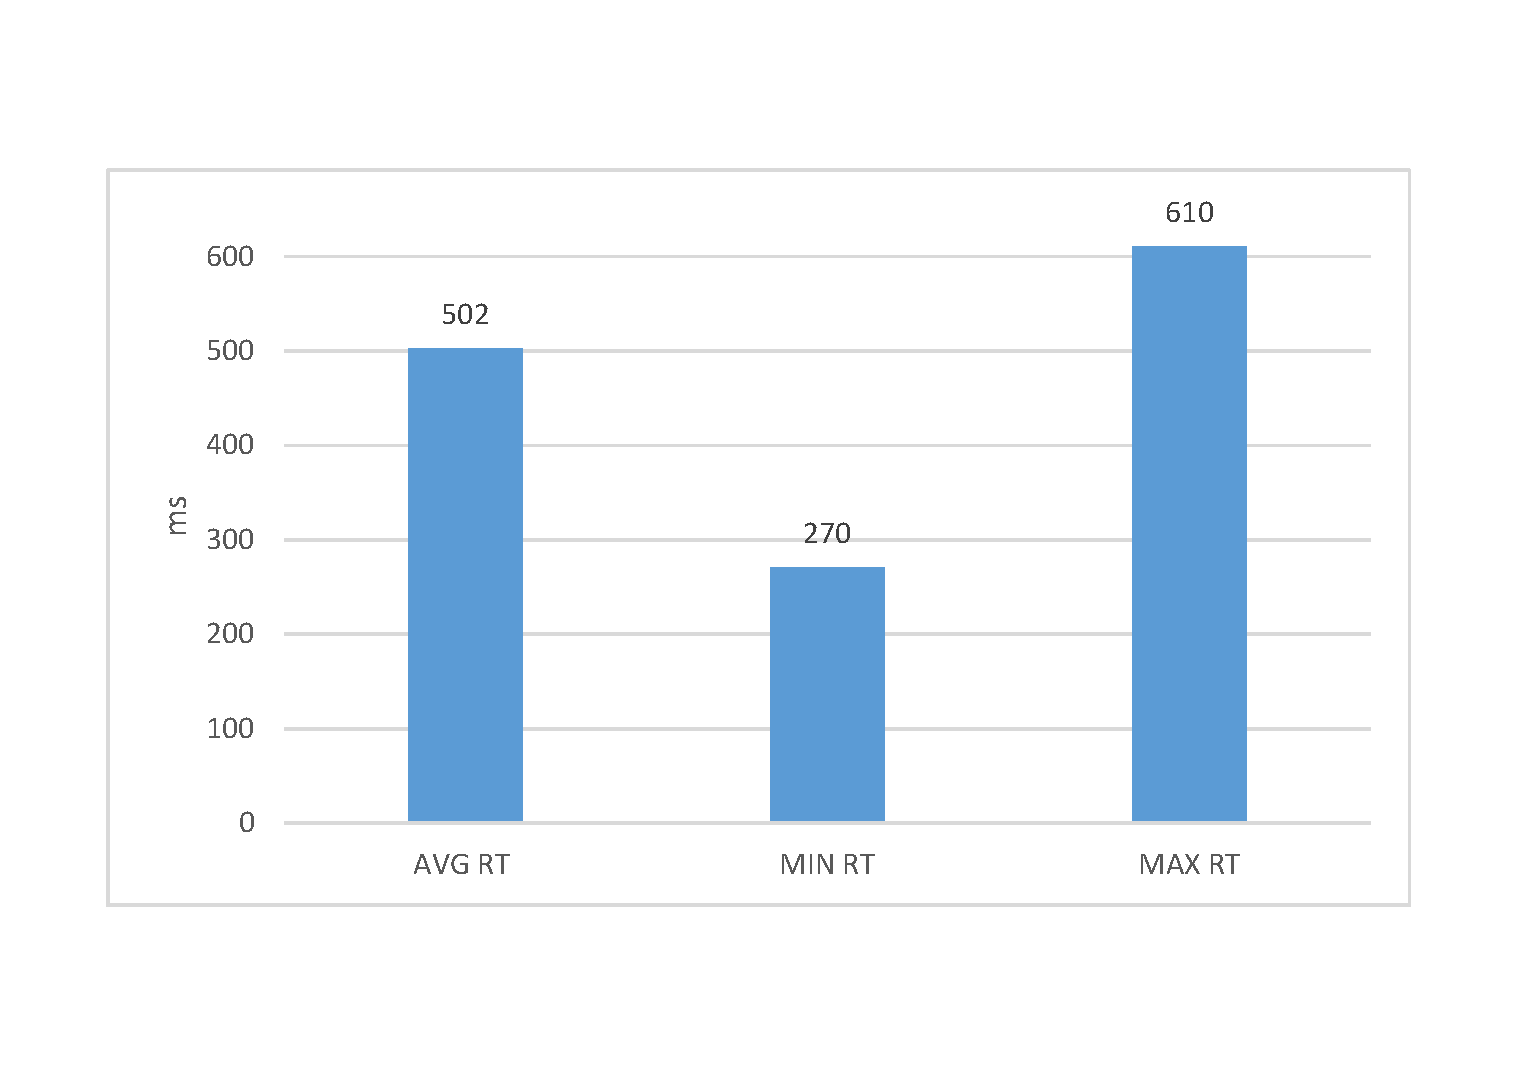
\includegraphics[width=0.8\textwidth,natwidth=200,natheight=150]{./fig/RT2SN.pdf}
	\centering
	\label{fig:rt2SN}
\end{figure}

\begin{figure}[h]
	\caption{The CPU utilization for two Social Network Engines.}
	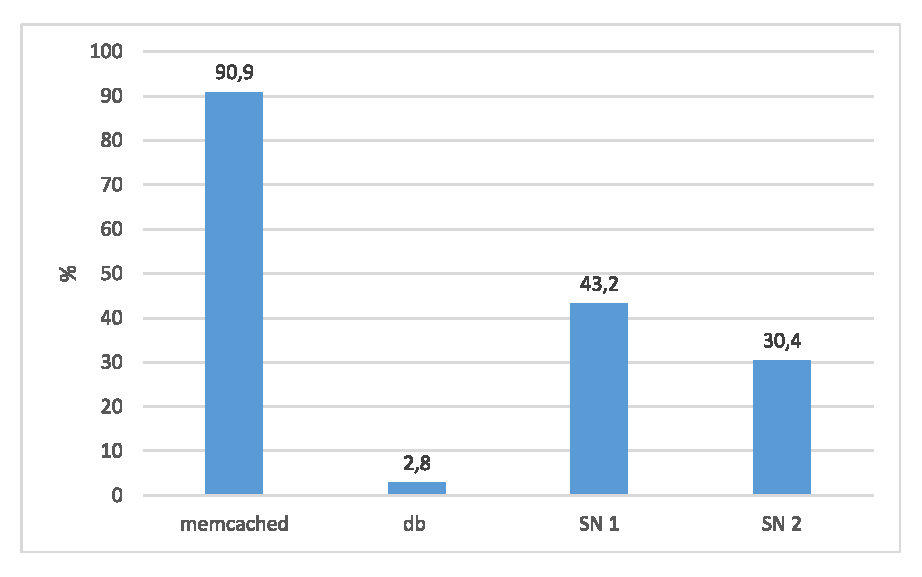
\includegraphics[width=0.8\textwidth,natwidth=200,natheight=150]{./fig/Usage2SN.pdf}
	\centering
	\label{fig:cpu2SNavg}
\end{figure}

This Section evaluates the horizontal scale of Social Network engine as described in~\ref{sec:engine_scale}. A memcached node was living between the Social Networking Engines and the back end system. The VM resources were kept the same as in the previous experiment and shown in the table~\ref{vms_resources}. One more Social Networking Engine instance was added with the same type as former SN Engine. 

So, the system architecture now consists of two Social Networking Engines as front-end. At the back-end of the system we have: (1) one Memcached node and (2) the CDO client - server, the Social Network Database and the CDO repocitory. The two SN Engines are deployed to a dedicated VM each. Furthermore, each SN Engine has its own CDO client deployed with them. The Memcached node is deployed on its own VM and the CDO Server, the Social Network Database and the CDO repository are deployed on the same VM.

The figure~\ref{fig:cpu2SNavg} shows the average CPU utilization for the Memcached, the MySql Database (db) and the two SN Engines (SN1, SN2). The load for this experiment is the same as the previous L3, which means we have ten users that request \emph{eight} applications for one hundred times consecutively. The first SN Engine has 43,2\% CPU usage and the second one has 12,8\% less. This difference is due to the first instance being deployed together with the NFS server and Apache Zookeeper on the same VM. 

With only one SN Engine the CPU Utilization was 57,09\% and now with two SN Engines the CPU Utilization is reduced to 43,2\%. This reduction is due to the requests being distributed to two instances instead of the only one instance. The CPU Utilization of the Memcached node increased, but this can be solved by introducing more Memcached nodes as the previous Section describes. Furthermore, we can introduce more SN Engines to support more heavy loads.

Since, the load from one SN Engine is now distributed to two SN Engines instances, the response time improved for the Load 3, as shown in the figure~\ref{fig:rt2SN} compared to the previous test-bench. The best achieved RT of previous architecture was 992 ms and with this architecture it reduced to 502 ms.

We can combine the two architectures together, meaning that we have more than one SN Engine and more than one Memcached to support as many loads as we want.

\section{Topic classification}
\label{sec:nlp_evaluation}
This Section evaluates the topic classification tool as described in Section~\ref{sec:natural_implementation} for the first training set. This set had five different classes or, according to StackOverflow dialect, five tags, as described in~\ref{sec:natural_implementation} and shown in table~\ref{table:nlp_eval}. For the testing set, thirty questions from StackOverflow were used per class. Those questions were different from the training set and had the highest activity during that specific time period. Each row at table~\ref{table:nlp_eval} shows a class as classified by StackOverflow users, and each column shows how our classifier classifies the question. For example, twenty one questions about \emph{reliability} were classified correctly, but eight were wrongly classified as \emph{optimization} and one was wrongly classified as \emph{performance}. The misclassification however, was not an error of our classifier. The reason of these mistakes is that  some questions from the testing set were either wrongly classified by the StackOverflow users or had more than one tags. For example, one question that was wrongly classified as \emph{performance} instead of \emph{reliability} was: ``can somebody explain me how to handle errors. my code is: \ldots''. The above question is out of the scope of reliability and even though the user tagged it as a reliability question, it was downvoted and marked as ``very low quality'' from the StackOverflow community.

Another example showing that the classifier is not misclassifying, but the problem stands in the users' tagging, is the following question:
``I want to perform some data manipulation tasks and analysis in spark and want to \textbf{optimize} the run times. 
here is the problem: \ldots ''. 
This question was marked by the user with both scalability and optimization tags. Even though this question is retrieved with the scalability tag and in the table it is shown as a wrong classification, after examining this question, one can realize that the \emph{scalability} tag was wrongly added by the user and only the \emph{optimization} tag should be placed.

This shows that our tool can further be used by StackOverflow to mark new questions that are wrongly tagged or misguided. There is a trend among StackOverflow users to add as many tags as they can in order to attract the attention of other users, increase the views of their question and finally get their answers.  

The true positive, which means a document is recognized in the correct class, according the table~\ref{table:nlp_eval} is 85. The false positive, which means a document is not correctly recognized, of this topic evaluation is 65. According to those precision metrics the accuracy or sensitivity of our topic classifier for this specific experiment is 56,67\%.

\begin{table}[]
\centering
\caption{NLP Evaluation of Classification}
\label{table:nlp_eval}
\begin{tabular}{|l|c|c|c|c|c|}
\hline
class / class & \multicolumn{1}{l|}{reliability} & \multicolumn{1}{l|}{design} & \multicolumn{1}{l|}{optimization} & \multicolumn{1}{l|}{performance} & \multicolumn{1}{l|}{scalability} \\ \hline
reliability   & \textbf{21}                    & 0                           & 8                                 & 1                                & 0                                \\ \hline
design        & 2                                & \textbf{17}               & 6                                 & 3                                & 2                                \\ \hline
optimization  & 2                                & 3                           & \textbf{16}                     & 8 & 1                                \\ \hline
performance   & 1                                & 1                           & 11                                & \textbf{16}                     & 1                                \\ \hline
scalability   & 6                               & 3                           & 3                                 & 3                                & \textbf{15}                     \\ \hline
\end{tabular}
\end{table}

\section{Requirements and user interface}
\label{eval_ui}
The User Interface of social networking platform is designed through the iterative process of several expert-based evaluations being carried out in group sessions. To obtain additional feedback from non-experts, three additional user-based evaluation experiments were designed and carried out involving potential users and presented in~\cite{magoutis2015design}. 

The author collaborated in the expert-based evaluations sessions focusing on the platform user interface design. Furthermore, the contributions of the author, in the user interface evaluations, was to make the platform support them and also author took part in the third evaluation process.  

The first experiment, carried out by Flexiant Ltd. aimed at assessing the overall look and feel of the network, the navigation mechanisms, as well as the design of fundamental functionality.

The second evaluation experiment, carried out by HCI team, aimed to collect subjective results rather than performance metrics. It involved another set of 12 users who, after a brief introduction to the available facilities, were asked to use the interactive prototype~\cite{Virzi1996} using the free exploration method of the Thinking Aloud protocol~\cite{jordan1998introduction} and fill-in a questionnaire in order to rate and comment their experience. 

The third evaluation experiment involved 15 participants who were guided through the interactive prototype of the PaaSage social network using specific scenarios. They were interviewed on their requirements and feedback following a semi-structured interview approach [84]. The evaluation session was carried out via Skype. Participants were recruited through European companies and organizations associated with the PaaSage EU project~\cite{paasage}. They were either developers or operations staff, thus within the target user groups of the PaaSage social network. Participants were not users of the PaaSage platform; some however were familiar with the project’s goals and objectives. Before the experiment, each participant was requested to fill-in a background information form and was sent an informed consent form, explaining all the recording and anonymity-ensuring procedures. 

\begin{figure}[h]
	\caption{SNP features that were mostly liked by the users.}
	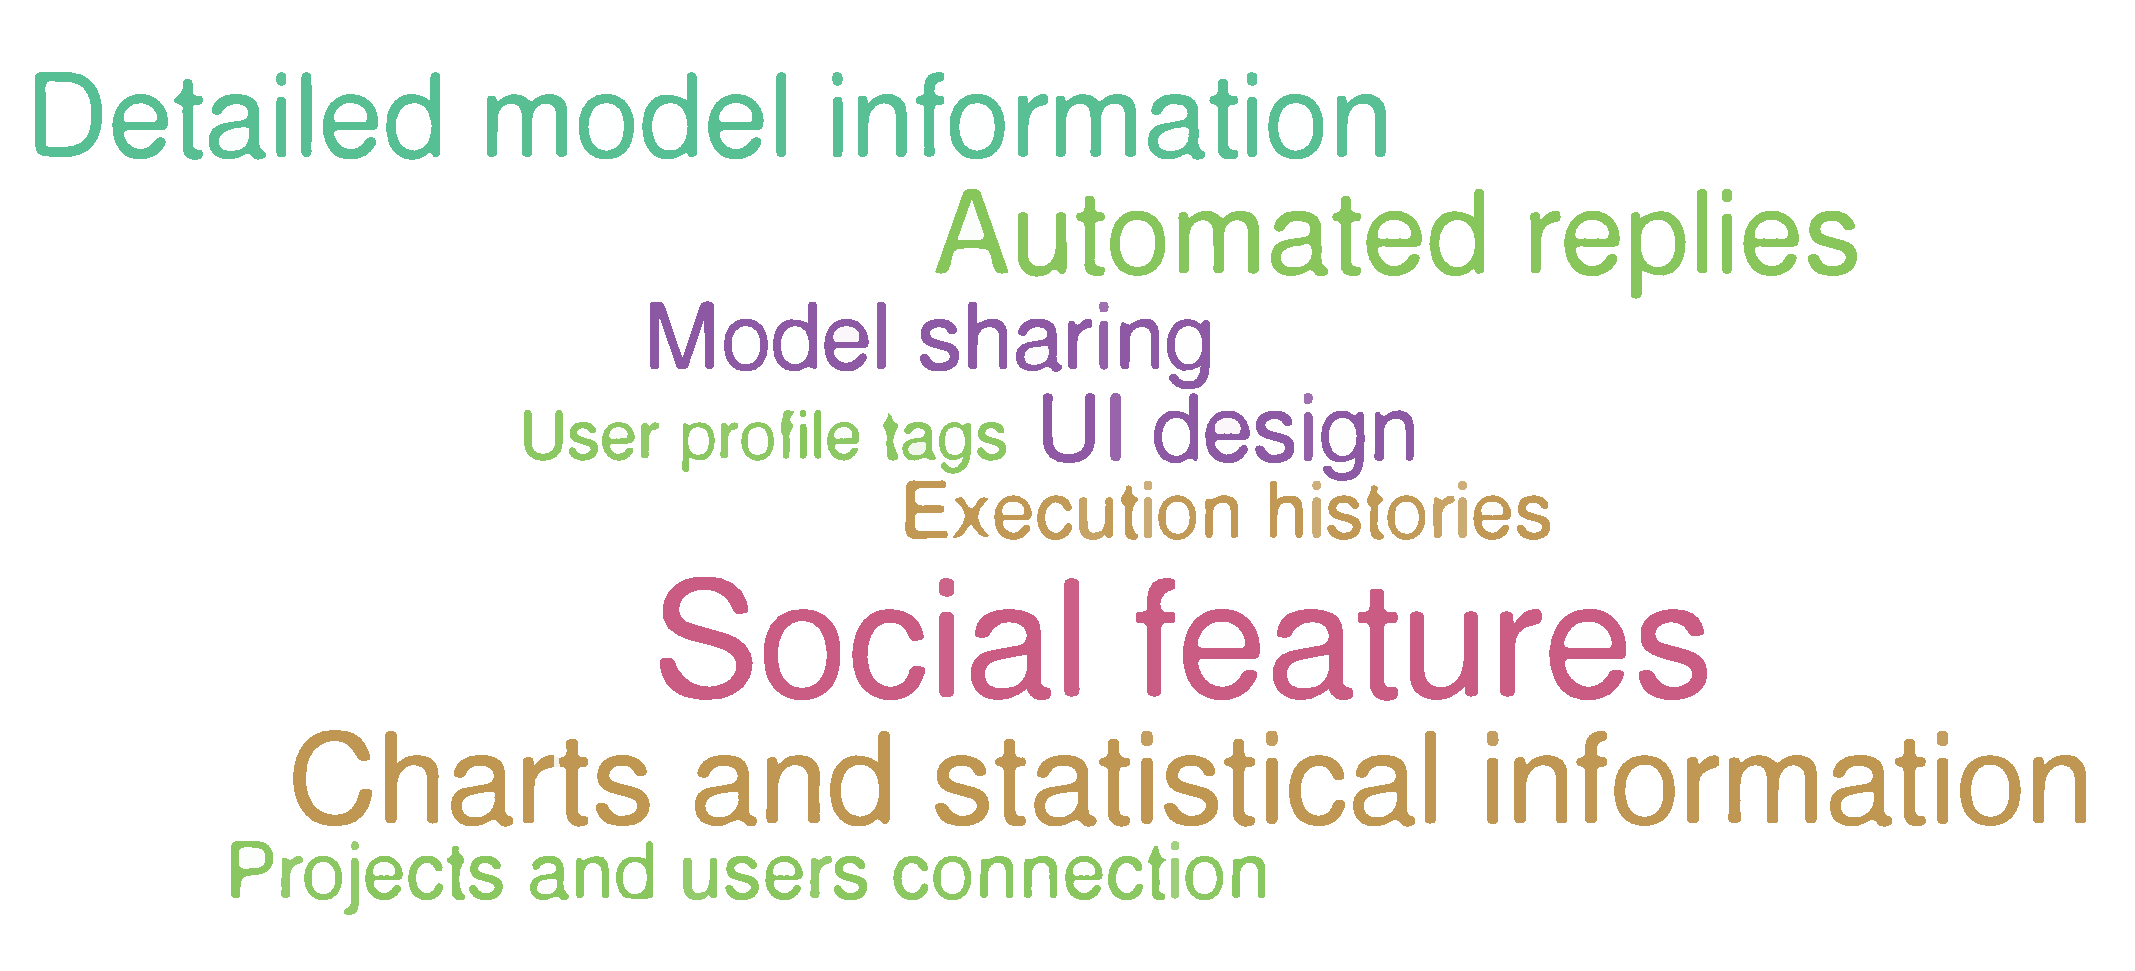
\includegraphics[width=1\textwidth,natwidth=200,natheight=150]{./fig/most-liked.pdf}
	\centering
	\label{fig:most-liked}
\end{figure}

Users, in the third experiment, were asked to identify up to three most-liked and three most-disliked features. Most-liked features presented in figure~\ref{fig:most-liked} included: the employment of social features in a development environment; the use of charts and statistical information to represent data; the detailed model information that could be retrieved and the model execution histories; the automatically-generated hints provided by the network as replies in discussion topics; the concept of sharing one’s models; the overall UI design; the direct connection between projects and users, and the user profile tags that allowed them to find users that would be interesting to connect with.

Those evaluation experiments show that a platform that couples together the employment of social networking features in community-building activities with the DevOps demands about application deployment, the execution analysis, the automatically generated hints based on data analysis is a helpful tool that people would like to use.